\chapter{Materiales y Métodos}

Se utilizó el repositorio de datos de los trabajos de grado de la biblioteca Alberto Quijano Guerrero de la universidad de Nariño. 

En este capítulo se describen los procesos de construcción, limpieza y transformación
del corpus de documentos de los trabajos de grado. Luego se detallan los experimentos
realizados; con el objetivo de descubrir relaciones conceptuales en el corpus de trabajos
de grado de la Universidad de Nariño utilizando la metodología CRISP-DM.



\section{Comprensión del problema}

En esta fase, se realizaron las actividades que permitieron profundizar y apropiar de una manera completa el problema objeto de estudio, los objetivos y los requisitos de esta investigación,
 que posibilitaron la recolección de los datos correctos para interpretar adecuadamente los resultados. En esta fase, descubrir las relaciones conceptuales del repositorio de documentos no estructurados de trabajos de grado de la universidad de Nariño,
 se convirtió en un problema a resolver con minería de textos.  Como resultado de la fase de compresión se construyó un marco teórico de diferentes técnicas de minería  de textos para abordar el problema; contemplado en el capítulo anterior.

\section {Comprensión de los datos}

En esta fase, se identificó, recopiló y familiarizó con el corpus de trabajos de grado, disponible en el repositorio de la biblioteca Alberto Quijano Guerrero de la universidad de Nariño.
Se construyó un repositorio inicial donde se integraron todos los trabajos de grado de los diferentes programas de la universidad de Nariño. Dando como resultado un repositorio compuesto por 8.076 documentos no estructurados, el cual sirvió de base para las subsiguientes fases. 

\section{Preparación de los datos}
En la fase de preparación se realizó el pre procesamiento del corpus primero que todo se descartó de los textos la sección de agradecimientos,
 utilizando expresiones regulares; se obtuvo las secciones de resumen, introducción, marco teórico, metodología, resultados y conclusiones.
 Después de eliminar la sección de agradecimientos se eliminaron las palabras muertas de la colección usando la librería Spacy de Python,
 seguidamente se lematizaron las palabras del corpus, ejemplo desarrollo por desarrollar.  Obteniendo como resultado un corpus limpio y listo para el desarrollo del trabajo. La figura  \ref{fig:proceso1} detalla el proceso de pre procesamiento del corpus.

\begin{figure}[H]
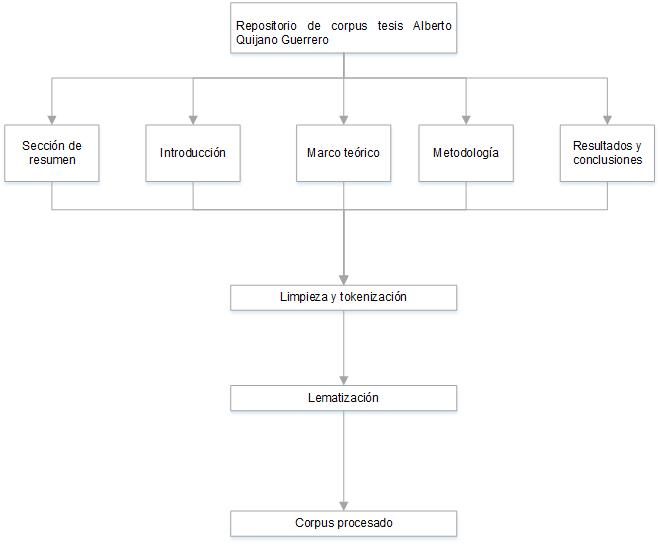
\includegraphics[width=1\textwidth]{proceso1}
\caption{Flujo de trabajo para el armado del corpus}
\label{fig:proceso1}
\end{figure}



\section{Modelado}

Una vez organizado el corpus se implementaron diferentes técnicas de minería de texto; para obtener diferentes conjuntos de datos estructurados .
Para estructurar documentos se usaron tres técnicas diferentes, las dos primeras proveniente de la librería Sklearn; CountVectorizer (Bow) y TfidfVectorizer (TF-IDF); la tercera técnica utilizada fue Doc2vec proveniente de la librería Gensim. 


\textbf{Modelos Bow y TF-IDF}

A continuación, se describen los parámetros establecidos para la generación de los modelos Bow y TF-IDF de la librería Sklearn; los cuales comparten los mismos parámetros.
\begin{itemize}
	\item Max\_df: Al construir el vocabulario, ignora los términos que tienen una frecuencia de documento estrictamente más alta que el umbral dado (palabras vacías específicas del corpus). Este parámetro toma un rango devalores [0, 1]. Para nuestro caso se usó en 0.7, ignorando los términos que estén presentes como mínimo en el 70\% de los documentos. 
	\item Min\_df: Al construir el vocabulario, ignora los términos que tienen una frecuencia de documento estrictamente más baja que el umbral dado. Este valor también se llama corte en la literatura. Toma valores en el rango de [0, 1], el parámetro representa una proporción de documentos, recuentos enteros absolutos. Paranuestro caso se elige 0.01;
		 eliminando términos que solo aparecen en el 1\% delos documentos.
	\item Ngram\_range: Límite inferior y superior del rango de valores n para los diferentes n-gramas que se van a extraer. Por ejemplo, un ngram\_range de (1, 1) utilizara solo unigramas, (1, 2) utilizará unigramas y bigramas, y (2, 2) utilizara solo bigramas. Para nuestro caso se usó (1,2) generando unigramas y bigramas.
	\item Max\_features: Máximo número de variables a generar. Para nuestro caso se generaron  2 modelos con 10.000 y 20.000 variables.

\end{itemize}


\textbf{Modelos Doc2vec}

A continuación, se describen los parámetros establecidos para el entrenamiento de los modelos Doc2vec PV-DBOW y PV-DM de la librería Gensim; los cuales comparten los mismos parámetros.

\begin{itemize}
  \item Dm: Esto define el algoritmo de entrenamiento. Por defecto  (dm = 1), se utiliza memoria distribuida (PV-DM). De lo contrario, una bolsa distribuida de palabras (PV-DBOW) es empleado, para nuestro caso se usó los  dos métodos propuestos  por el modelo doc2vec dm=0 y dm=1 
  \item Size: Tamaño del vector de salida para la representación un documento, se eligió 20.
  \item Window: Esta es la distancia máxima entre la palabra predicha y el contexto de palabras utilizadas para la predicción dentro de un documento, se eligió un valor de 10.
  \item Alpha: Esta es la tasa de aprendizaje inicial (caerá linealmente a min\_alpha a medida que el entrenamiento progresa), se eligió 0.025.
  \item Min\_count: Ignora todas las palabras con una frecuencia total inferior a esta, se eligió 50 para limitar el tamaño del vocabulario a palabras significativas. Se ignora cualquier palabra que aparezca menos de 50 veces.
\end{itemize}

Para iniciar el análisis, se verifica si existe tendencia al agrupamiento en cada uno de los conjuntos de datos estructurados por los modelos generados anteriormente. Utilizamos el estadístico de Hopkins para establecerlo, recurrimos al paquete RANN de R. Seleccionamos 1000 puntos al azar de los datos de muestra y luego se los compara con 1000 puntos creados al azar. Luego se calcula la distancia al vecino más cercano de ambas muestras y finalmente se establece el estadístico para cada conjunto de datos.  La figura  \ref{fig:proceso2} detalla el proceso.

\begin{figure}[H]
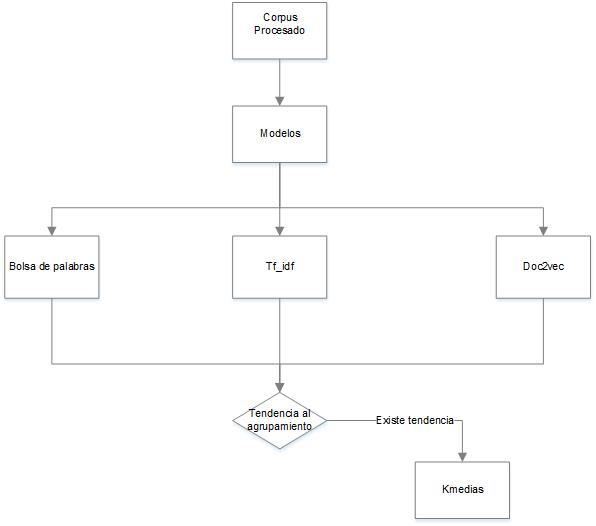
\includegraphics[width=1\textwidth]{proceso2}
\caption{Flujo de trabajo para la generación de un conjunto de datos estructurado }
\label{fig:proceso2}
\end{figure}

%
%
%La tabla \ref{tab:ProgramasDM} muestra el estadístico de Hopkins para cada conjunto de datos generado. 
%
%
%\begin{table}[H]\centering
%	\caption{Descripción de la tendencia al agrupamiento en los conjuntos de datos.}\label{tab:ProgramasDM}
%	\begin{tabularx}{\textwidth}{XXXm{6.0cm}}\toprule
%
%Modelo &  \multicolumn{1}{c}{Estadístico Hopkins} & \multicolumn{1}{c}{Descripción} \\ 
%Bow & 0.61 & Modelo Bow generando un conjunto de datos de 10.000 filas * 20.000 
%columnas usando unigramas y bigramas.
%Este método descarta términos que aparezcan en más del 70\% de documentos.  \\ 
%Bow &  0.58 & Modelo Bow generando un conjunto de datos de 10.000 filas * 10.000 
%columnas usando unigramas y bigramas.
%Este método descarta términos que aparezcan en más del 70\% de documentos.   \\ 
%Tf-idf & 0.54 & Modelo Tf-id generando un conjunto de datos de 10.000 filas * 20.000 
%columnas usando unigramas y bigramas.
%Este método descarta términos que aparezcan en más del 70\% de documentos.  \\ 
%Tf-idf &  0.52 & Modelo Tf-id generando un conjunto de datos de 10.000 filas * 10.000 
%columnas usando unigramas y bigramas.
%Este método descarta términos que aparezcan en más del 70\% de documentos.   \\ 
%Doc2vec & 0.38 & Este método representa un documento mediante 
%un vector de tamaño 20
%usando el algoritmo bolsa de palabras distribuida  (PV-DBOW)   \\ 
%Doc2vec & 0.42  & Este método representa un documento mediante
%un vector de tamaño 20
%usando el algoritmo memoria distribuida (PV-DM) \\  \bottomrule
%	\end{tabularx}
%
%\end{table}
%
%Con un umbral establecido en 0.5 podemos confirmar que existe tendencia al agrupamiento en los conjuntos de datos generados por los modelos Doc2vec bolsa de palabras distribuida (PV-DBOW) y Doc2vec memoria distribuida (PV-DM).
%%Los resultados muestran una mejor tendencia al agrupamiento en los modelos Doc2vec,
%Los modelos Doc2vec  logran captar relaciones conceptuales mediante el contexto que representa cada documento, usando esta representación se podrá medir qué tan relacionado está un documento con respecto a los demás.	

\textbf{Agrupación}

La agrupación es un ejercicio popular de aprendizaje automático, y las técnicas utilizadas en las tareas de clustering clásicas pueden utilizarse para texto una vez estructurado, con la idea de formar grupos de trabajos de grado de acuerdo a su dominio de conocimiento, para posteriormente entrenar el modelo word2vec en cada grupo o área específica encontrada. Para determinar la cantidad de grupos óptimos (K) se corrió el algoritmo kmedias para diferentes K, variando desde 20 hasta 44. Se calculó la suma de errores al cuadrado (SSE) y el coeficiente de Silhouette para cada valor de K. SSE mide la distancia de los puntos al centroide por lo cual esperamos que SSE sea lo más bajo posible. El coeficiente de Silhouette es útil para analizar la cohesión y la separación del agrupamiento, valores cercanos a 1 indican que el agrupamiento es bueno, valores alrededor de cero o hasta negativos indican que el k no es el óptimo o la tendencia al agrupamiento no es tan buena. Para la tarea de agrupación se usó la librería sklearn de Python y el algoritmo kmeans en los conjuntos de datos estructurados con tendencia al agrupamiento. 


%\begin{figure}[H]
%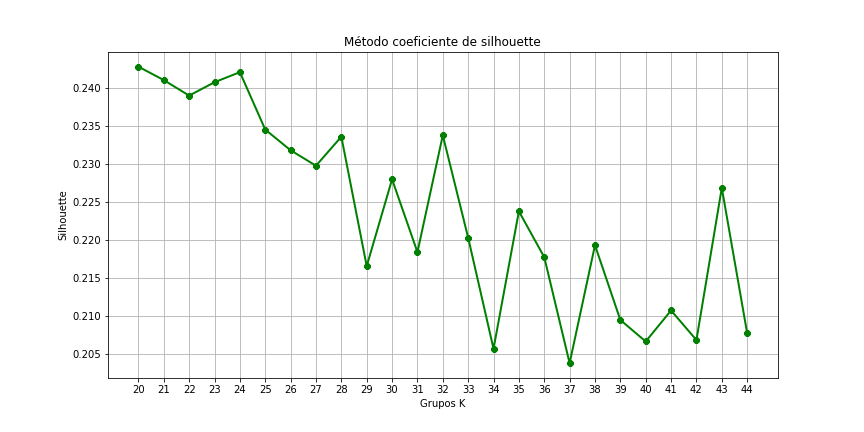
\includegraphics[width=1\textwidth]{Silhouette}
%\caption{Método coeficiente de Silhouette algoritmo Kmedias }
%\label{fig:proceso3}
%\end{figure}
%
%\begin{figure}[H]
%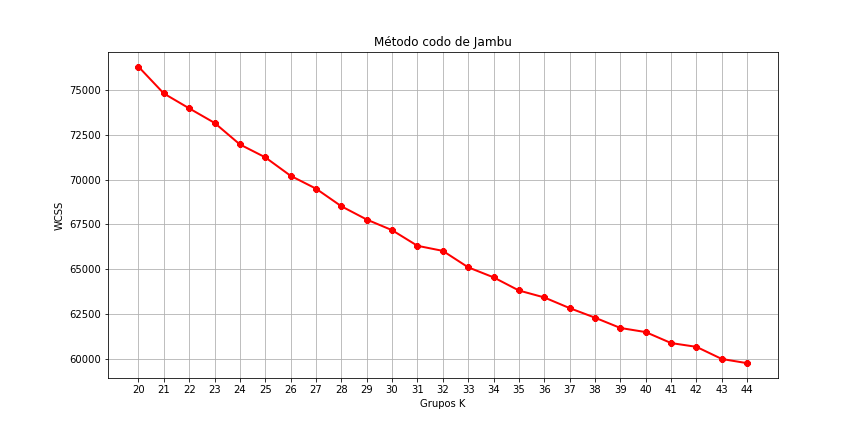
\includegraphics[width=1\textwidth]{WCSS}
%\caption{Método de codo de Jambu algoritmo Kmedias}
%\label{fig:proceso4}
%\end{figure}
%
%En la figura  \ref{fig:proceso3} se visualiza el método de coeficiente de Silhouette; el cual sugiere que el número adecuado de grupos es de 24, en la figura  \ref{fig:proceso4} se visualiza el método del codo de Jambu; 
%para el cual miramos que a medida que k se incrementa la distancia de los puntos al centroide va disminuyendo. Para la selección del K óptimo  se contrasto los dos métodos y se eligió el k en 32; ya que miramos que su coeficiente de Silhouette está entre los más altos y a la vez la distancia de los puntos al centroide es baja. 

\textbf{Modelo Word2vec}

Por cada grupo encontrado se entrenó el modelo Word2vec, con el fin de encontrar relaciones conceptuales entre los términos de dominio presentes en los documentos. 
Para este proceso se configuró un cluster con Apache Spark con el fin de paralelizar el entrenamiento y acelerar el tiempo de procesamiento, se utilizó la librería Pyspark para la programación en paralelo y la librería Gensim para el entrenamiento del modelo Word2vec y como entrada el corpus de lemas clasificado por su respectivo grupo encontrado.


Se utilizaron los siguientes parámetros para el entrenamiento:

\begin{itemize}
  \item	SG: Define el algoritmo de entrenamiento. Por defecto (sg = 0), se utiliza continuous bag of words (CBOW). De lo contrario (sg = 1), se emplea skip-gram, Skip-gram es más lento, pero produce mejores resultados por lo cual se eligió (sg=1).
  \item	Window: esta es la distancia máxima entre la palabra actual y la predicha dentro de una oración, se eligió 10.
  \item	Size: Este es el tamaño de los vectores que representan a un término, Valores razonables son entre 10 y cientos, se eligió 200.
  \item	Alpha: Esta es la tasa de aprendizaje inicial (caerá linealmente a min\_alpha a medida que el entrenamiento progresa), se eligió 0.03.
  \item	Min\_count: Ignora todas las palabras con una frecuencia total inferior a esta, se eligió 50 para limitar el tamaño del vocabulario a palabras significativas. Se ignora cualquier palabra que aparezca menos de 50 veces.
  \item	Workers: Número de núcleos a utilizar para el procesamiento del trabajo. Para el caso se utilizó todos los núcleos disponibles de la máquina.
  \item	hs: Si es 1, softmax jerárquico se utilizará para el entrenamiento del modelo. Si se establece en 0 (predeterminado), y negativo es distinto de cero, se utilizará un muestreo negativo, se eligió 1 softmax jerárquico.
  \item	Iter: Este es el número de iteraciones (épocas) sobre el corpus. El valor establecido para el caso fue 6000.
\end{itemize}

\textbf{Clasificación}

Para clasificar futuros trabajos que se ingresen a Maskana se entrenaron varios modelos de aprendizaje supervisado, donde la clase a aprender es el grupo o categoría encontrada por el algoritmo k-medias y las variables predictoras son los vectores generados por el algoritmo Doc2vec.
La figura \ref{fig:procesocalsificacion} detalle el proceso de entrenamiento de los diferentes modelos de aprendizaje supervisado.


\begin{figure}[H]
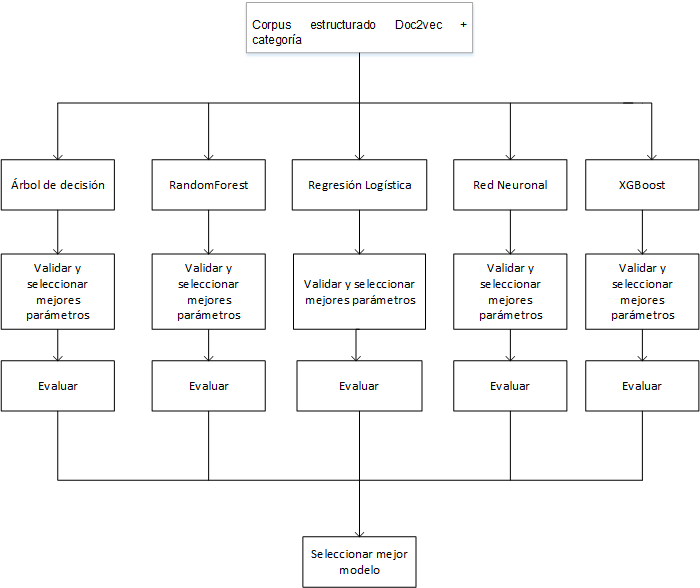
\includegraphics[width=0.9\textwidth]{procesocalsificacion}
\caption{Flujo de trabajo para el entrenamiento de modelos de aprendizaje supervisado.}
\label{fig:procesocalsificacion}
\end{figure}

Para el entrenamiento de estos modelos se usó el módulo mlib de la librería pyspark. Para cada modelo de clasificación, se implementó una grilla  de búsqueda para iterar sobre los  hiperparámetros  mediante el método de validación cruzada y la métrica de accuracy (exactitud).

A continuación se detalla la selección de los  parámetros de cada modelo:

\textbf{Árboles de decisión}

\begin{itemize}
	\item MaxDepth: Profundidad máxima del árbol. Se itero este parámetro con valores de  [3, 5, 10, 15, 20], el mejor resultado se lo obtuvo con maxDepth=5.
	\item MinInstancesPerNode: Número mínimo de instancias que debe  recibir un nodo para dividirse. Se itero este parámetro con valores de  [5, 10, 15, 20, 50], los mejores resultados se obtuvieron con minInstancesPerNode=10. 
	\item Impurity: Medida de impureza utilizada para elegir entre posibles divisiones. Se itero sobre los dos posibles valores de este parámetro ['entropy','gini'], se obtuvieron mejores resultados con impurity= 'entropy'.
\end{itemize}

\textbf{RandomForest}

\begin{itemize}
	\item NumTrees: Número de árboles en el bosque aleatorio .Se itero con valores de [100,500,1000], los mejores resultados se obtuvieron con numTrees=500.
	\item MaxDepth:Profundidad máxima de los árboles del bosque aleatorio. Se itero con valores de  [3, 5, 10, 15, 20], los mejores resultados se obtuvieron con maxDepth=10.
	\item MinInstancesPerNode: Número mínimo de instancias que debe  recibir un nodo para dividirse. Se itero este parámetro con valores de  [5, 10, 15, 20,50], los mejores resultados se obtuvieron con un valor de minInstancesPerNode=5. 
	\item Impurity: Medida de impureza utilizada para elegir entre posibles divisiones. Se itero sobre los dos posibles valores de este parámetro ['entropy','gini'], se obtuvieron mejores resultados con impurity= 'gini'.
	\item MinInfoGain: Para que un nodo se divida aún más, la ganancia de información que genera la división debe superar el valor mínimo establecido.Se itero con valores de   [0.0, 0.25, 0.5, 0.75],  se obtuvieron mejores resultados con minInfoGain=0.25
\end{itemize}

\textbf{Regresión Logística}
\begin{itemize}
	\item Max\_iter: Número máximo de iteraciones que se toman para que los solucionadores converjan. Se itero este parámetros con [10.000, 20.000], se obtuvo mejores resultados con  max\_iter=10.000.
	\item Penalty: Se utiliza para especificar la norma utilizada en la penalización. Se itero con ['l1', 'l2'], obteniendo mejores resultados con penalty= 'l1'.
	\item Class\_weight: Pesos asociados a las clases del entrenamiento. Si no se da, se supone que todas las clases tienen un peso uno. El modo 'balanceado' usa los valores de la variable Y, para ajustar automáticamente los pesos inversamente proporcionales a las frecuencias de clase en los datos de entrada como n\_samples / (n\_classes * np.bincount (Y)). Se itero este parámetros con [none,'balanced']; alcanzando un mejor resultado con  class\_weight='balanced'
\end{itemize}

\textbf{Red Neuronal}



\begin{itemize}
	\item La capa de entrada consta de 20 neuronas para las variables de entrada generadas por el modelo Doc2vec.
	\item En la capa de salida se configuró 32 neuronas, una  por cada categoría encontrada.
	\item En las capas de entrada y capas ocultas se usó la función de activación logsig y en la capa de salida la función softmax.
	\item Para el entrenamiento de la red neuronal se probó y validó diferentes arquitecturas  [20, 1 , 32], [20, 5 , 32] , [20, 10, 32], [20, 10, 10, 32] y [20, 15, 15, 32].
	\item La arquitectura que mejor resultados obtuvo fue [20, 10, 10, 32]; 20 neuronas de entrada, 2 capas ocultas con 10 neuronas interconectadas y 32 neuronas en la capa de salida. 

\end{itemize}

\textbf{XGBoost}

\begin{itemize}
	\item N\_estimators: Número de árboles con aumento de gradiente, Se definió este parámetro en 500.
	\item Learning\_rate: El parámetro learning\_rate se puede configurar para controlar la ponderación de los árboles nuevos agregados al modelo y así evitar el sobreajuste. Se itero con valores de [0.3, 0.1,  0.01], Se obtuvo  mejores resultados con learning\_rate= 0.3.
	\item Max\_depth: Profundidad máxima de un árbol. Incrementar este valor hará que el modelo sea más complejo y más probable que se sobreajuste.se itero este parámetro con [3 , 5, 10 ,20] logrando mejores resultados con  max\_depth=3
	\item Booster: Algoritmo a utilizar. Puede ser gbtree, gblinear o dart; gbtree y dart usan modelos basados en árboles, mientras que gblinear usa funciones lineales. Para nuestro caso Booster= gblinear obtuvo mejores resultados.
	\item Min\_child\_weight: Suma mínima de peso de instancia necesaria en un nodo hijo. Si el paso de la partición del árbol da como resultado un nodo hoja con la suma del peso de la instancia menor que min\_child\_weight, entonces el proceso de construcción dejará de particionar el árbol. Se itero con los valores de [1, 5, 10, 15, 20], obteniendo mejores resultados con min\_child\_weight=1. 
\end{itemize}

\section{Evaluación}

En esta fase se evaluaron los modelos generados con el fin de determinar su validez, seleccionar los mejores parámetros de cada modelo y así implementarlos dentro de la herramienta Maskana.  La evaluación de los modelos se describe en los capítulos de Resultados y Discusión.



\section{Implementación}

En esta fase se implementaron los algoritmos utilizados en esta investigación en la herramienta Maskana, con el fin de que cualquier usuario pueda encontrar relaciones conceptuales en los trabajos de grado consultados en esta herramienta.
Se usó el modelo Doc2vec entrenado en la fase anterior para la detección de documentos conceptualmente relacionados, además para cada búsqueda realizada por el usuario en Maskana se implementó la opción de encontrar temas o tópicos referentes a los documentos relacionados y usando el modelo Word2vec entrenado con el conocimiento de cada documento del repositorio se generó un grafo conceptual para su visualización. 

Todo el proceso de construcción fue realizado bajo el sistema operativo Debian 10. Se utilizó los lenguajes de programación Python 3.7 y Java.
Maskana está compuesta por 3 módulos: el módulo GUI, el módulo núcleo y el módulo de conexión. en esta fase se implementó un cuarto módulo denominado servicios de minería de texto, el cual se describe en el capítulo de Resultados.
El código del proyecto se encuentra en el siguiente repositorio  \textcolor{Cyan}{\underline{\url{https://github.com/jimaguere/relaciones-conceptuales/tree/master}}}

% el cual se puede observar en la  figura \ref{fig:implementacion1}.

%
%
%\begin{figure}[H]
%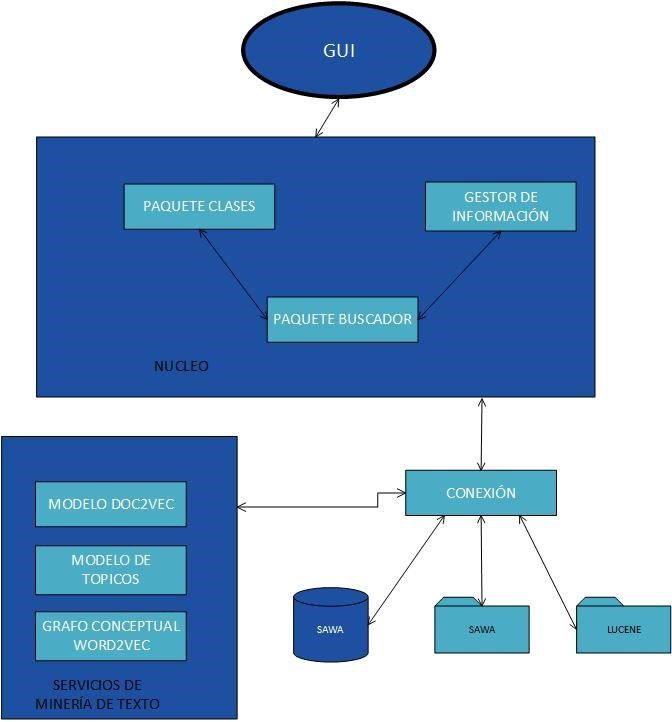
\includegraphics[width=0.9\textwidth]{implementacion1.png}
%\caption{Arquitectura de Maskana.}
%\label{fig:implementacion1}
%\end{figure}
%
%\textbf{Módulo de Servicios de Minería de texto.}
%
%Este módulo es el encargado de brindar servicios web que conectan a Maskana con los modelos elaborados en la sección de modelado, en este módulo
% se encuentran los algoritmos para relacionar documentos conceptualmente,
% conocer los temas o tópicos principales de los trabajos de grado consultados y sus relaciones.
% A continuación, se hace una descripción de los submódulos que lo componen.
%
%\textbf{Modelo Doc2vec:}
%Este submódulo lleva el nombre del modelo Doc2vec,el cual se encarga de realizar la representación vectorial de todos los documentos del repositorio, generando vectores conceptuales teniendo en cuenta el contexto de los documentos con los que fue entrenado, estos vectores están almacenados en la base de datos Sawa mediante el módulo de conexión, 
%se implementó el algoritmo \ref{alg:maskanita1} , el cual permite  encontrar similitudes conceptuales entre los documentos del repositorio; ayudando a extender las búsquedas que realizan los usuarios de la herramienta Maskana.
%
%\begin{algorithm}
%    \renewcommand{\algorithmicrequire}{\textbf{Input:}}
%    \renewcommand{\algorithmicrequire}{\textbf{Input:}}
%    \renewcommand{\algorithmicensure}{\textbf{Output:}}
%    \renewcommand{\algorithmicprint}{\textbf{break}}
%  \caption{ Maskanita recomendación de trabajos de grado.}
%  \label{alg:maskanita1}
%  \algsetup{indent=2em}
%  \footnotesize
%  \begin{algorithmic}[1]
%\REQUIRE {D: documento resultado de búsqueda} 
%\REQUIRE {Corpus\_doc2vec : corpus estructurados con el modelo doc2veca} 
%\ENSURE {DocRel: conjunto de documentos relacionados a D}
%\STATE $DocRel \leftarrow \emptyset$
%\STATE vector\_documento=doc2vec(D)
%\STATE grupo\_documento=xgboost.clasificar(vector\_documento)
%\FOR {each doc  \in$ Corpus\_doc2vec  \in$  grupo\_documento }
%	\IF{ similitud\_coseno( vector\_documento,doc2vec(doc))>0.7}
%		  \STATE {DocRel $\leftarrow $adicionar(DocRel,doc) }
%		% \STATE {D $\leftarrow$ points $\in c$ }
%	\ENDIF
%\ENDFOR
%\STATE {ordenar(DocRel) }
%\end{algorithmic}
%\end{algorithm}
%
%%\begin{figure}[H]
%%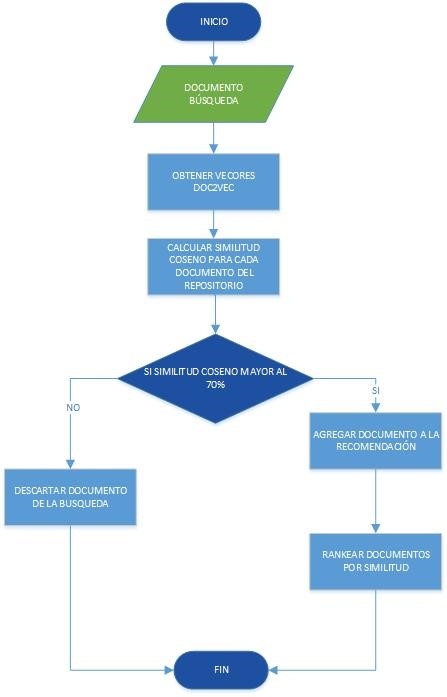
\includegraphics[width=0.7\textwidth]{implementacion2}
%%\caption{Diagrama de flujo algoritmo Maskanita recomendación de trabajos de grado.}
%%\label{fig:implementacion2}
%%\end{figure}
%
%\textbf{Modelo de tópicos:} En este submódulo se encuentra implementado el algoritmo LDA para conocer los diferentes tópicos 
%o temas relacionados con los trabajos de grado, recomendados por el algoritmo Maskanita. Como primer paso se toma los documentos recomendados por el algoritmo Maskanita, como segundo paso 
%se obtiene el número de temas a calcular por parte del usuario, seguidamente se ejecuta el algoritmo LDA de la librería Gensim de Python, 
%Finalmente se obtienen los temas principales que componen los documentos recomendados y se los visualiza mediante el servicio web de este submódulo.
%
%\begin{figure}[H]
%\centering
%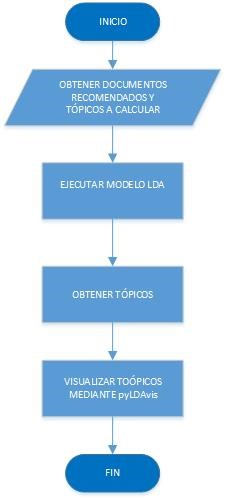
\includegraphics[width=0.3\textwidth]{implementacion3}
%\caption{Proceso submódulo modelo de tópicos.}
%\label{fig:implementacion3}
%\end{figure}
%
%
%\textbf{Grafo conceptual Word2vec:} En este submódulo se encuentra implementado  el algoritmo \ref{alg:maskanita2}, útil para representar relaciones conceptuales del contenido de los trabajos de grado recomendados por el algoritmo Maskanita  \ref{alg:maskanita1}. 
%El primer paso toma como entrada los documentos recomendados por Maskanita \ref{alg:maskanita1}, En segundo lugar, se obtiene conceptos relevantes de los documentos de entrada mediante la tarea de reconocimiento de entidades nombradas de la librería Spacy de Python,
%Para cada entidad o concepto reconocido se aplica el modelo Word2vec para conocer sus relaciones, finalmente se construye el grafo conceptual usando la librería D3.js y  el servicio web implementado en este submódulo.  
%
%
%\begin{algorithm}
%    \renewcommand{\algorithmicrequire}{\textbf{Input:}}
%    \renewcommand{\algorithmicensure}{\textbf{Output:}}
%    \renewcommand{\algorithmicprint}{\textbf{break}}
%  \caption{ Maskanita relaciones conceptuales de trabajos de grado.}
%  \label{alg:maskanita2}
%  \algsetup{indent=2em}
%  \footnotesize
%  \begin{algorithmic}[1]
%\REQUIRE {T: contenido textual documentos relacionados } 
%\ENSURE {G: Grafo Conceptual }
%\STATE $conceptos\_ner \leftarrow \emptyset$
%\STATE $G \leftarrow \emptyset$
%\STATE {spacy.load('es\_core\_news\_sm') }
%\FOR {each token  \in$ T }
%	\IF{spacy.isNer(token)}
%		  \STATE {$conceptos\_ner $\leftarrow $adicionar(conceptos\_ner,token)}
%		% \STATE {D $\leftarrow$ points $\in c$ }
%	\ENDIF
%\ENDFOR
%
%\FOR {each c  \in$ conceptos\_ner }
%	\FOR {rl  \in$  word2vec.sim(c) }
%		  \STATE {$n1 $\leftarrow $crearNodo(c)}
%		  \STATE {$n2 $\leftarrow $crearNodo(rl)}
%		  \STATE {$G $\leftarrow $relacionarNodos(n1,n2)}
%	\ENDFOR
%\ENDFOR
%
%
%\end{algorithmic}
%\end{algorithm}

%%%%%%%%%%%%%%%%%%%%%%%%%%















